\newcommand{\texCommand}[1]{\texttt{\textbackslash{#1}}}%

\newcommand{\exemplo}[1]{%
\vspace{\baselineskip}%
\noindent\fbox{\begin{minipage}{\textwidth}#1\end{minipage}}%
\\\vspace{\baselineskip}}%

\newcommand{\exemploVerbatim}[1]{%
\vspace{\baselineskip}%
\noindent\fbox{\begin{minipage}{\textwidth}%
#1\end{minipage}}%
\\\vspace{\baselineskip}}%

%%%%%%%%%%%%%%%%%%%%%%%%%%%%%%%%%%%%%%%%%%%%%%%%%%%%%%%%%%%%%%%%%%%%%%%%%%%%%%%%
%%%%%%%%%%%%%%%%%%%%%%%%%%%%%%%%%%%%%%%%%%%%%%%%%%%%%%%%%%%%%%%%%%%%%%%%%%%%%%%%
%%%%%%%%%%%%%%%%%%%%%%%%%%%%%%%%%%%%%%%%%%%%%%%%%%%%%%%%%%%%%%%%%%%%%%%%%%%%%%%%
Essa seção apresenta o contexto necessário para descrever a abordagem proposta: Seção \ref{sec:datastreams} Explica sobre problemas de fluxos de dados e como lidar com mudança de conceito e retreinamento. 
Seção \ref{sec:metalearning} apresenta a abordagem MtA, incluindo o processo de construção dos meta-dados e como recomendar algoritmos. 
A Seção \ref{sec:metastream} descreve o MetaStream, um sistema de recomendação de algoritmos, baseado em MtA, para fluxos de dados.

\section{Fluxos de Dados}
\label{sec:datastreams}
Dados estáticos e bem estruturados não se apresentam como uma boa alternativa em ambientes com massiva interação livre de usuários, uma das possíveis abordagens para esses ambientes são fluxos de dados.
\textcolor{red}{CARACTERIZAR AQUI FLUXOS DE DADOS, diferenças para series temporais, explicar sazonalidade}
A maioria das técnicas de AM assumem que os dados são independentes e identicamente distribuídos (\textit{iid}),
mas essas premissas geralmente não se sustentam em ambientes de fluxos de dados, como apontado por A. Bifet and R. Gavald\`a (2007) \cite{bifet2007learning},
dado que os dados chegam interminavelmente e, por isso, podem apresentar dependência temporal e mudanças de conceito pode ocorrer.
Outro aspecto critico é a imposição de limites computacionais a esses ambientes, como memória, CPU, e largura de banda \cite{bifet2010moa, gama2012survey}.
Para resolver esses problemas, diversas tecnologias foram desenvolvidas. Dentre elas, as mais proeminentes são mecanismos de esquecimento, testes estatísticos e algoritmos adaptativos.

Mecanismos de esquecimento fazem dados recentes tornarem-se mais relevantes e dados passados menos, um exemplo são janelas deslizantes \cite{gaber2005mining}, um método agnóstico de modelo. 
Sistemas baseados em testes estatísticos agem monitorando uma métrica pre-definida, tal como performance preditiva do modelo, e então ``disparam'' um alarme quando a qualidade dessas métricas está abaixa de algum limiar tolerável, demandando alguma ação.

Exemplos dessa abordagem são o teste de Page-Hinkley e o \textit{Statistical Process Control} \cite{gama2010knowledge}.
Baseado nessas duas soluções, o \textit{ADaptive WINdowing} (ADWIN) \cite{bifet2007learning} usa testes estatísticos para definir o tamanho de cada janela, ajustando ao ``tamanho do conceito''.
Entretanto, embora esses métodos serem capazes de alarmar uma redução na performance dos modelos e adaptar o tamanho da janela a isso, não é possível identificar os algoritmos ou modelos que se tornaram mais apropriados ao novo conjunto de dados que está sendo gerado.

Algoritmos de aprendizado adaptativo, como o VFDT \cite{domingos2000mining},
foram inicialmente introduzidos com fluxos de dados em mente, desempenhando aprendizado online e baixo consumo de memoria, mas não conseguiam se adaptar a mudança de conceito, um problema já conhecido na época.
Mais tarde, aprimoramentos foram propostos, como o CVFDT (um aprimoramento direto sobre o VFDT) \cite{hulten2001mining}, o HAT \cite{bifet2009adaptive} e o ARF \cite{gomes2017adaptive}, que podem lidar com variação de conceito aplicando janelas deslizantes sobre o processo de treinamento.
Entretanto, se a mudança for muito abrupta, o espaço de hipótese, fixado a priori do algoritmo (Arvore de Decisão (AD) para a maioria deles) pode não ser mais adequado e as adaptações desejadas não serem atingidas.
Esses problemas podem ser reduzidos quando se usa detectores de mudança baseado em sistemas de recomendação baseados em MtA, almejando espaços de hipótese como tarefas de aprendizado \cite{rossi2014metastream}.

\section{Meta-Aprendizado}
\label{sec:metalearning}
O problema de seleção de algoritmos foi inicialmente observado por J. R. Rice (1976) \cite{Rice1976} com o principal objetivo de prever o melhor algoritmo para resolver um dado problema quando houver mais de um algoritmo que resolva disponível.
Os componentes desse modelo são: o espaço de instâncias do problema ($P$), que é composto por conjuntos de dados em MtA; o espaço de instâncias de atributos ($F$), que são os meta-atributos usados para descrever os conjuntos de dados; o espaço de algoritmos ($A$), que contém um conjunto de algoritmos de AM que podem ser recomendados; e um espaço de medidas de avaliação ($Y$), responsável por recuperar as performances dos algoritmos de AM que resolvem as instâncias dos problemas contidos em $P$.
Usando os conjuntos anteriores, o sistema MtA pode obter um algoritmo capaz de mapear um conjunto de dados $p$, descrito pelos meta-atributos $f$, em um (ou mais) algoritmo $\alpha$ capaz de resolver o problema com um performance boa, de acordo com $y$, por exemplo, com máximo $y(\alpha(p))$.

K. A. Smith-Miles (2008) \cite{SmithMiles2008} 
aprimorou esse modelo abstrato propondo generalizações que podem também ser aplicadas ao problema de projeto de algoritmos.
Nessa proposta, alguns componentes são adicionados: o conjunto de algoritmos de MtA; a generalização de regras empíricas ou ranqueamento de algoritmos; a verificação de resultados empíricos, que podem ser guiados por uma base teórica ao aprimoramento de algoritmos.

Um componente crucial dos modelos anteriores é a definição do conjunto de meta-atributos ($F$) usados para descrever propriedades gerais dos conjuntos de dados.
Esses meta-atributos devem ser capaz de prover evidências sobre performance futuro dos algoritmos em $A$ \cite{Soares2001, Reif2012}
e discriminar, com baixo custo computacional, a performance de um grupo de algoritmos.
Os principais meta-atributos usados na literatura de MtA podem ser divididos em cinco grupos: Gerais, Estatísticos, Teoria da Informação, Baseados em Modelo e Landmarkings.

Os gerais podem ser facilmente extraidos dos dados \cite{Reif2014}, com baixo custo computacional \cite{Reif2012}.
Os meta-atributos estatísticos capturam os indicadores principais sobre localização e distribuição dos dados, tais como média, desvio padrão, correlação e curtose.
Meta-atributos de teoria da informação, usualmente medidas de entropia \cite{Segrera2008}, capturam a quantidade de informação em um (sub)conjunto dos dados \cite{SmithMiles2008}.
Já os baseados em modelo são propriedades extraídas de modelos de AM, geralmente AD \cite{Bensusan2000, Peng2002}, induzidos dos dados sob analise \cite{Reif2014}.
Os meta-atributos de Landmarking usam a performance de algoritmos de aprendizado simples e rápidos para caracterizar os conjuntos de dados \cite{SmithMiles2008}. 

A definição do conjunto de instâncias de problema ($P$) é outra preocupação, quando o ideal seria usar um grande número de conjuntos de dados diversos, com objetivo de induzir um meta-modelo confiável.
Para reduzir o viés dessa escolha, conjuntos de dados de diversos repositórios, tais como o UCI\footnote{\url{https://archive.ics.uci.edu/ml/index.php}} \cite{Lichman2013} e o OpenML\footnote{\url{http://www.openml.org/}} \cite{OpenML2013}, podem ser usados.

O espaço de algoritmos $A$ representa o conjunto de algoritmos candidatos a serem recomendados no processo de seleção de algoritmos.
Idealmente, esses algoritmos devem também ser suficientemente distintos entre si e representar toda a região do espaço de algoritmos \cite{Munoz2018}. 
Os modelos induzidos pelo algoritmo podem ser avaliados por diferentes medidas, para tarefas de classificação, a maioria dos estudos usando MtA usam acurácia. Entretanto, outros indicadores, como o $F_\beta$, AUC e coeficiente Kappa, também podem ser usados.

Após a extração dos meta-atributos dos conjuntos de dados e a mensuração da performance do conjunto de algoritmos nesses conjuntos de dados, o próximo passo é rotular cada meta-exemplo nos meta-dados. 
Brazdil et al. (2009) \cite{Brazdil2009} resume as quatro propriedades principais frequentemente usadas para rotular meta-exemplos em MtA: ($i$)
o algoritmo que apresenta a melhor performance no conjunto de dados (uma tarefa de classificação); ($ii$) o ranqueamento dos algoritmos de acordo com suas performances no conjunto de dados (uma tarefa de ranqueamento), onde o algoritmo com melhor performance está no topo do ranque; ($iii$) o valor de performance obtido por cada algoritmo individualmente no conjunto de dados (uma tarefa de regressão) e; ($iv$) a descrição do modelo, que é geralmente baseado em agrupamentos ou regras de associação.

Em ambientes de fluxos de dados, o espaço de instância de problemas é composto por apenas um problema $p$ enquanto os meta-atributos $F$ são extraídos dos dados de cada janela temporal para compor o meta-exemplo.
É importante que o processo de extração dos meta-atributos tenha baixo custo computacional e alto grau de informação.
Além disso, a  performance desses algoritmos $A$ são obtidas periodicamente, usualmente para cada janela deslizante. 
Portanto, o algoritmo atual é substituído logo que o meta-modelo prediz que um algoritmo diferente é mais adequado para os exemplos da próxima janela deslizante.
Essa é uma abordagem padrão na literatura de MtA em fluxos de dados \cite{read2012batch, vanrijn2014algorithm, Anderson2019}.

Nesse trabalho, é apresentado um método baseado em MtA que segue o framework MetaStream \cite{rossi2014metastream}.
A ideia básica é tentar selecionar o melhor algoritmo para ambientes que mudam com o tempo.
Para tal ambiente, o MetaStream regularmente induz um meta-classificador capaz de mapear as características extraídas de dados passados e os que estão chegando à performance dos classificadores nesses dados.
Diferente de trabalhos anteriores, um conjunto de meta-atributos mais inovadores baseado em A. Rivolli et al. (2018) \cite{Rivolli2018} é aplicado e uma abordagem de aprendizado incremental no nível meta é aplicada usando o LightGBM \cite{ke2017lightgbm}.

\section{Metastream}
\label{sec:metastream}

A literatura apresenta alternativas a seleção de algoritmos (ou modelos) baseado em MtA para mudança de conceito. Um dos primeiros a apresentar é R. Klinkenberg (2005) \cite{klinkenberg2005}, onde características obtidas do processo de aprendizado em si, no caso o tamanho das janelas deslizantes, foram usadas para induzir meta-modelos.
Uma abordagem diferente foi investigada por J. Gama and P. Kosina (2014) \cite{gama2014} e R. Anderson et al. (2019) \cite{Anderson2019}
reusando modelos previamente aprendidos mas usando o mesmo algoritmo para induzir esses modelos no fluxo de dados. Uma terceira alternativa é dada por J. N. van Rijn et al. (2018) \cite{VanRijn2018}, onde é usado conjuntos de modelos, tendo um alto custo computacional para induzir modelos para cada algoritmo e manter os pesos atualizados.

Em seguida, é apresentado o MetaStream baseado no trabalho de A. L. D. Rossi et al. (2014) \cite{rossi2014metastream}, que tem fases ``offline'' e ``online''.
A fase offline is projetada para escolha de hiper-parâmetros, validação e treinamento e geração dos dados em lote.
A fase online age no ambiente dinâmico, recomendando um algoritmo para uma dada janela de dados. Ambas as fases são baseadas em sistemas de recomendação de MtA.


\subsection{Offline Phase}
\label{subsubsec:offline}

%\andre{As soon as the minimum amount of training data arrives, i.e., a batch of training data becomes available, ...}

%This phase begins by waiting for a reasonable amount of training data to arrive. 
With the batch of data already available, the base-algorithms are induced through $K$-fold cross-validation.
After that, in a sliding window setting, as shown in Figure \ref{fig:ms_diag0_off}, a $\omega_{b1}$ window is used to induce models using the base-level algorithms and the meta-features $x^m$ are also extracted from this window. %and the label of this meta-example represents the . 

\begin{figure}[ht]
    \centering
    \includegraphics[width=\linewidth]{img/ms_diag0_off.svg}
    \caption{Meta-feature extraction from $\omega_b$ and label obtaining from
    $\eta_b$ windows.}
    \label{fig:ms_diag0_off}
\end{figure}

Then, the induced models are evaluated on the examples of the $\eta_{b1}$ window, where the best model is the one with the greater predictive performance. Thus, the meta-example is labeled as $y^m$, which represents the algorithm that induced the best model. This generates the first meta-example. The same process is applied $N$ steps further, where $N$ is the minimum number of instances to induce a consistent model, 
to generate the initial meta-data, where the first model to apply in the online phase is induced.

\subsection{Online Phase}
\label{subsec:online}

In the online phase, the algorithm received a continuous stream of data. 
At first, it gets a feature vector  %of predictive attributes 
$\boldsymbol{x}_b = (x_1,...,x_p)$, and with some delay, the target attribute $y_b \in \{0,1,..,k\}$ for classification, where $k$ is the number of classes.
%At first, it gets a vector of predictive attributes $\boldsymbol{x}_b = (x_1,...,x_p)$, and with some delay later, the target attribute $y_b \in \{0,1,..,k\}$ for classification or $y_b \in \rm{I\!R}$ for regression.

Figure \ref{fig:ms_diagram0} shows the time $t$ of the online phase. 
It has a window of fixed size $\omega_b$ that will be used to induce a model, a window of fixed size $\eta_b$ where the model induced on $\omega_b$ will be evaluated as soon as the target values are discovered, a $\gamma_b$ range which is the delay to observe the target attribute for the examples in $\eta_b$ window and a variable size $\lambda_b$ of examples waiting to be processed.
When $\gamma_b$ is the same size as $\eta_b$, that is, all target values in $\eta_b$ were obtained, the $\omega_b$ window is shifted $\eta_b$ instances to right and a new model is induced in this window.

\begin{figure}[ht]
    \centering
    \includegraphics[width=\linewidth]{metastream_diag0}
    \caption{Window discretization at base-level data stream.}
    \label{fig:ms_diagram0}
\end{figure}

MtL comes to play in the second level of processing, named meta-level. As shown in Figure \ref{fig:ms_diagram1}, the meta-features are extracted from $\omega_b$ windows and generate a meta-example without the target value, which is kept for a later update. 

\begin{figure}[ht]
    \centering
    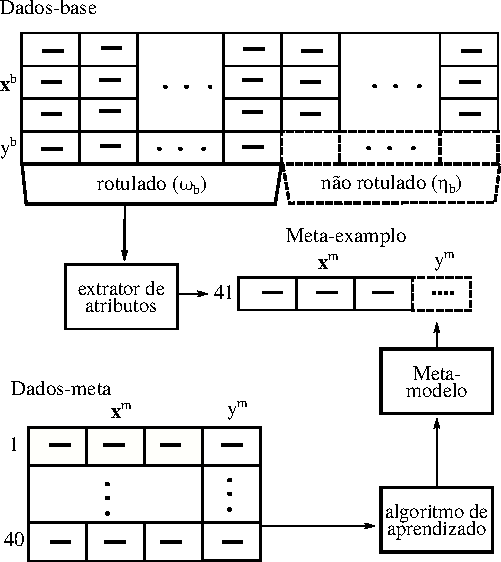
\includegraphics[width=\linewidth]{metastream_diag1}
    \caption{Meta-feature extraction from $\omega_b$ and $\eta_b$ windows at meta-level.}
    \label{fig:ms_diagram1}
\end{figure}

The learning algorithm (meta-model) uses previously labeled meta-examples in the meta-base to induce a meta-classifier, which is applied to recommend an algorithm to induce a model using the $\omega_b$ window that likely will be the most accurate to  predict the labels of the $\eta_b$ examples.
 




% Motivar IA, surgimento, historia,
%Em ambientes reais, a possibilidade de ações possíveis, cresce exponencialmente
%em função da complexidade da tarefa \cite{OpenAI2019,Silver2017}. Descrever
%instruções para que um automato lide de forma ótima nesses ambientes é, do ponto
%de vista prático, impossível. Diversos organismos apresentam dispositivos capazes
%de lidar com ambientes complexos sem analisar todo o espaço de ações possíveis
%\cite{shettleworth2001animal}, onde memorização, raciocínio e planejamento 
%fornecem uma solução quasi-otima para tais problemas.

%\section{Aprendizado de Máquina}
%\label{sec:aprendizado-de-maquina}
%No contexto de inteligência artificial, o aprendizado, ou \textit{aprendizado de
%máquina} (AM), é o estudo e a concepção de agentes que melhoram o seu desempenho
%nas tarefas futuras de aprendizagem após fazer observações sobre o mundo
%\cite{russell2016artificial}. Formalmente definido como:
%\begin{definition}
%Um programa de computador (agente), \textit{aprende} de uma experiência
% $\boldsymbol E$ a respeito de alguma classe de tarefa $\boldsymbol T$ e medida
% de performance $\boldsymbol P$, se a performance na tarefa $\boldsymbol T$,
% medido por $\boldsymbol P$, melhora com a experiência
% $\boldsymbol E$ \cite{mitchell1997machine}.
% \end{definition}

% Esta é uma definição geral de aprendizado, neste trabalho, lidaremos com um tipo
% específico dentre os diversos possíveis \cite{mohri2018foundations}, o aprendizado
% supervisionado. No modelo supervisionado, a experiência $\boldsymbol E$ é um
% registro $\boldsymbol{x}=(x_1,x_2,...,x_n)$ e seu respectivo rotulo $y$, e a
% tarefa $\boldsymbol T$ consiste em atribuir um valor $\hat{y}$ para um
% $\boldsymbol{x}$ onde o $y$ real ainda não é conhecido, mas assumindo que será
% independente e identicamente distribuído (IID). Ou seja, queremos nos aproximar de
% uma $f(\boldsymbol{x}) + \epsilon = y$, de tal forma que ao mensuramos observações
% futuras de $f(\boldsymbol{x})$ por $\boldsymbol P$, o valor de 
% $\boldsymbol{P}(\hat{y},y)$, tenda ao valor dado pelo erro de Bayes ($\epsilon$),
% também considerado o erro irredutível, esse diferente de zero pois há ruído em
% $\boldsymbol{x}$ ou variáveis não mensuradas por $\boldsymbol{x}$ que
% contribuem para $y$ \cite{friedman2001elements, abu2012learning}.


% \subsection{Inferência Indutiva}
% Definimos anteriormente que queremos descobrir uma função $f(\boldsymbol{x})$
% que aproxime a experiência ($\boldsymbol{E}$) dada pelo par $(\boldsymbol{x},y)$,
% ou seja, queremos induzir uma hipótese que explique nossa observação, para
% inferirmos valores futuros. Porém para um número finitos de exemplos existem
% infinitas funções que interpolam perfeitamente todos esses pontos, mas para que se
% tenha um bom desempenho em tarefas futuras, tal função deve se aproximas da real
% função geradora, o que nos leva a pergunta: qual dessas funções deve ser escolhida?

% Um princípio comumente aceito para essa escolha, é o chamado \textit{"Navalha
% de Ockham"} \cite{blumer1990occam}, esse princípio diz que para duas hipóteses de
% igual poder explicativo, é preferível escolher a \textit{mais simples}. No inicio
% do desenvolvimento de técnicas de inferência indutiva, não havia uma definição
% formal do que seria uma hipótese "mais simples", em 1964 com o trabalho de
% Solomonoff \cite{solomonoff1964formal}, é concebido uma definição formal para
% o que seria esse principio: a máquina de Turing (MT) de menor comprimento que
% computa tal observação, esse do ponto de vista teórico é um sistema indutivo
% perfeito \cite{rathmanner2011philosophical}.

% Porém já se é conhecido que tal programa não é computável, pois escolher um
% programa de menor comprimento equivalente é mapeável a $\text{PARA}_{MT}$. Uma
% solução a esse problema é escolher em um espaço de hipóteses $\mathcal{H}$
% (programas), \textit{apriori} fixo, chamado viés, em que nesse, por diversas
% teorias \cite{vapnik2013nature,bartlett2002rademacher}, que são aproximações ou
% casos especiais da teoria de Solomonoff, é possível selecionar a hipótese
% mais simples que melhor explica o fenômeno.

% Valiant em 1984 \cite{valiant1984theory}, propõe a teoria provavelmente aproximadamente correto (PAC)

% COMO DEFINIR APRIORI O ESPAÇO DE BUSCA?

% NAO HÁ UM ALGORITMO QUE PERFORME MELHOR NO GERAL, NO FREE LUNCH


% Em \cite{goodfellow2016deep}, são listadas mas não limitadas à onze tarefas
% possíveis ao aprendizado supervisionado, para o problema proposto realizaremos
% duas dessas tarefas, a classificação e a classificação com valores faltantes.

% \subsection{Classificação}
% Esta tarefa $\boldsymbol{T}$ consiste em designar uma categoria para a entrada
% $\boldsymbol{x}$ dentro do conjunto finito $\mathcal K$ de $k$ categorias. Queremos 
% então aproximar a função $f:\mathbb{R}^n\longrightarrow \{1,...,k\}$, tal que, dado 
% um conjunto de entrada $\boldsymbol{x}$ a função designará um valor $y =
% f(\boldsymbol{x})$ onde $y \in \mathcal{K}$. Existem variantes desta tarefa, que
% não será abordada, onde ao invés de designar uma classe precisa à entrada
% $\boldsymbol{x}$, é dado um vetor de probabilidades sobre todas as classes de
% $\mathcal K$ \cite{goodfellow2016deep}.

% % colocar exemplo pratico aqui? cancer/não-cancer

% \subsection{Classificação com Valores Faltantes}
% Similar a classificação, a classificação com valores faltantes se diferencia por
% nosso vetor de entrada $\boldsymbol{x}$ não conter alguns de seus valores. Isso
% torna o problema mais difícil pois ao invés de, usualmente, mapearmos
% $\boldsymbol{x}$ em $y$, por uma única função $f$, devemos criar varias funções
% que mapeiam subconjuntos de $\boldsymbol{x}$ e compô-los de alguma forma que o
% $\hat{y}$ estimado por essa função seja próximo do
% $y \in \mathcal{K}$ \cite{goodfellow2016deep}.

% % FAZER UM DIAGRAMA SIMILAR AO LEARNING FROM DATA pagina 30

% \section{Fluxos de Dados e Mudança de Conceito}
% \label{sec:fluxos-de-dados-e-mudanca-de-conceito}
% Uma série temporal é um conjunto de observações obtidas sequencialmente no tempo
% \cite{box2015time,brockwell2016introduction,durbin2012time}, onde o eixo temporal
% costuma estar ligado a frequência em que esses dados são gerados, ex. meses, para
% as vendas mensais de uma loja ou mili-segundos, para as transações de ações na
% bolsa de valores. Sendo uma série temporal um processo estocástico indexado
% \cite{hamilton1994time}, esse pode apresentar dependências temporais devido seu
% processo gerador, eventos futuros são influenciados por eventos passados
% \cite{karlin2012first}. Neste trabalho iremos nos ater a formalização do modelo
% de \textit{espaço de estados} aditivo \cite{durbin2012time}.
% \begin{definition}
%     Uma série temporal é um conjunto de observações $S=\{x_1,...,x_n\}$ indexadas
%     por $n \in \mathbb{N}$.
% \end{definition}

% O aprendizado apresentado na seção \ref{sec:aprendizado-de-maquina} é do tipo
% indutivo, ele se baseia no axioma empiricista de que o futuro irá se comportar
% como o passado \cite{vickers2009problem}, estatisticamente, que os dados serão
% estacionários gerados de uma mesma função de probabilidade. Em ambientes
% complexos e com dependência temporal, essa premissa pode não ser verdadeira
% \cite{hulten2001mining}. Em fluxos de dados, que serão discutidos na seção
% \ref{sec:fluxo-de-dados}, é comum tal mudança, portanto é necessário desenhar
% sistemas capazes de se adaptar a essas condições \cite{gama2007learning}.

% As séries temporais embora tenham um comportamento caótico devido sua natureza
% estocástica costumam apresentar três padrões de comportamento; tendência,
% sazonalidade e ciclos, esse os quais serão explorados aqui a nível meta.

% \paragraph{Tendência}
% Uma tendência existe quando há um crescimento ou decrescimento de longo termo na
% série temporal \cite{hyndman2018forecasting}, não necessariamente linear. Ele
% pode estar atrelado a crescimentos (ou decrescimentos) econômicos e populacionais,
% como demanda eletricidade, smartfones, entre outros.

% \begin{figure}[h]
%     \centering
%     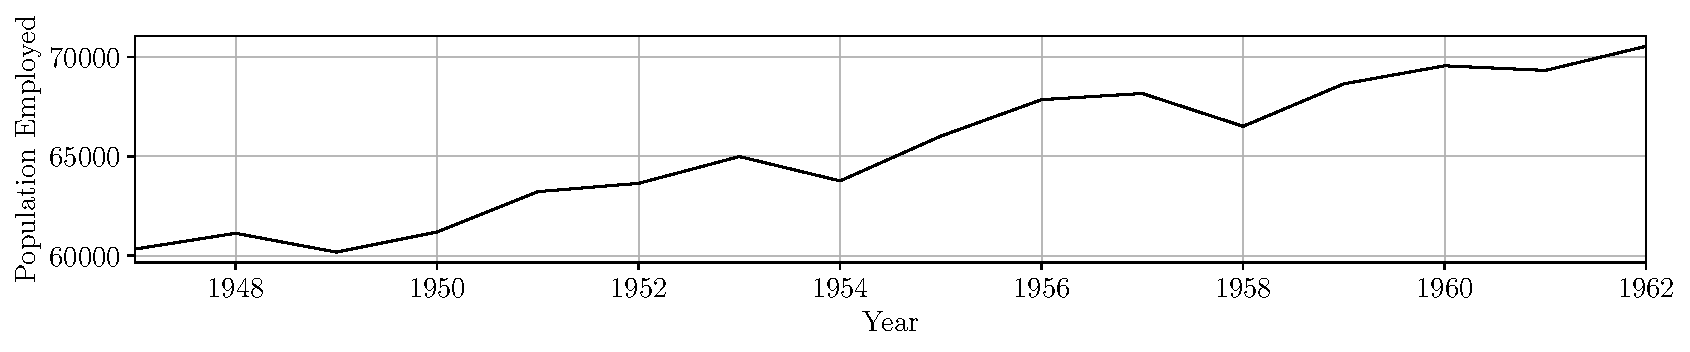
\includegraphics[width=1.0\textwidth]{img/longley.pdf}
%     \caption{Exemplo de tendência.}
%     \label{fig:trend}
% \end{figure}{}

% \equacao{trend}{y_t = \underbrace{\mu_t}_{\text{tendência}} +
% \sum_{i}^{k}{\underbrace{\beta_i x_{it}}_{\text{variáveis explicativas}}} + \epsilon}

% \paragraph{Sazonalidade}
% A sazonalidade é um padrão em séries temporais causado por fatores sazonais
% seguindo um período fixo de frequência conhecida, como dias, meses ou semestres
% \cite{hyndman2018forecasting}. Exemplo são vendas de ovos de Páscoa, casos de
% doenças transmitidas por insetos associados ao período de vida do mesmo.

% \begin{figure}[h]
%     \centering
%     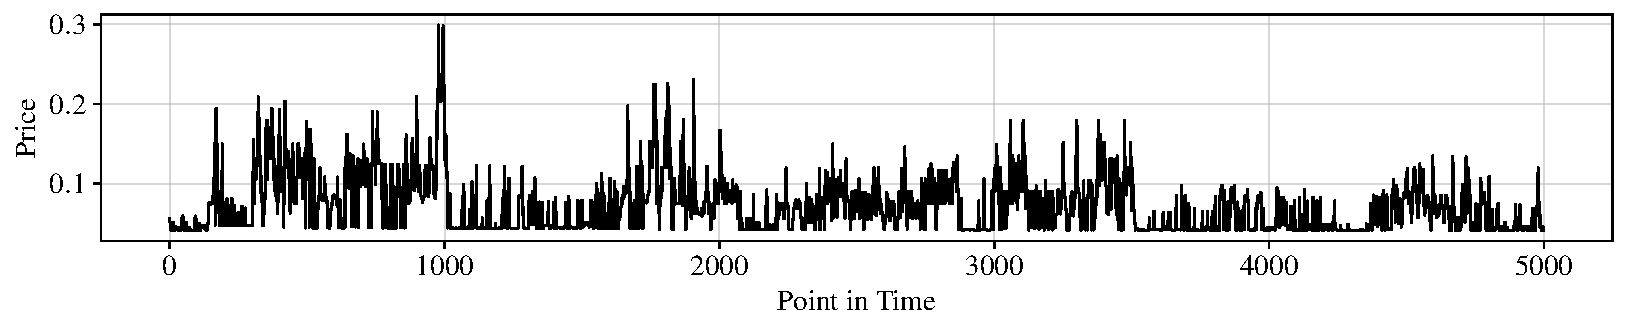
\includegraphics[width=1.0\textwidth]{img/elec.pdf}
%     \caption{Exemplo de sazonalidade.}
%     \label{fig:sazo}
% \end{figure}{}

% \equacao{seasonal}{y_t = \underbrace{\gamma_t}_{\text{sazonalidade}} +
% \sum_{i}^{k}{\underbrace{\beta_i x_{it}}_{\text{variáveis explicativas}}} + \epsilon}

% \paragraph{Ciclo}
% Um ciclo ocorre quando a série temporal exibe ascensões e quedas que não são de
% frequência fixa. Essas flutuações são usualmente devido a condições econômicas
% relacionadas a ``ciclos econômicos'' \cite{hyndman2018forecasting}.

% \begin{figure}[h]
%     \centering
%     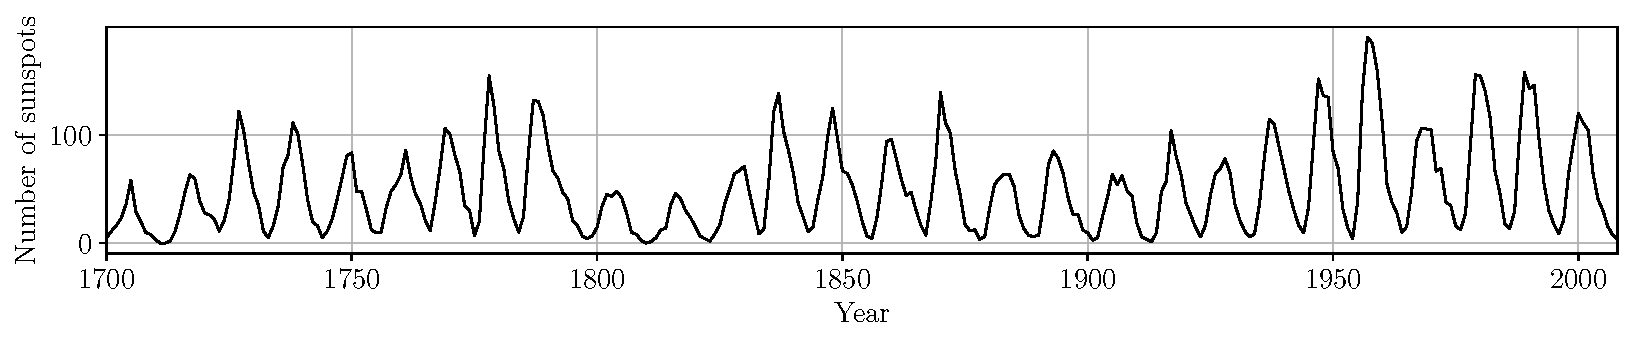
\includegraphics[width=1.0\textwidth]{img/sunspots.pdf}
%     \caption{Exemplo de ciclos.}
%     \label{fig:ciclo}
% \end{figure}{}

% \equacao{cycle}{y_t = \underbrace{c_t}_{\text{ciclo}} +
% \sum_{i}^{k}{\underbrace{\beta_i x_{it}}_{\text{variáveis explicativas}}} + \epsilon}

% %http://www.dfki.de/lwa2005/fgml/paper09.pdf mudança de conceito formal nesse paper


% \section{Mineração em Fluxo de Dados}
% \label{sec:fluxo-de-dados}
% Fluxo de dados, similar a series temporais, diferem conceitualmente por poderem
% ser lidos apenas uma ou poucas vezes, dado as limitações de computação e 
% armazenamento, e por não terem uma terminação\cite{gama2007learning}.
% \begin{definition}
%     Um fluxo de dados é um conjunto \textbf{infinito} de pares ordenados $D=\{(d_1,x_1),
%     (d_2,x_2),...,(d_t,x_t),...\}$, sendo $d_t$ um \textit{timestamp} e $x_t$ uma observação feita
%     no instante $d_t$.
% \end{definition}


% como
% apresentado na seção \ref{sec:series-temporais-e-mudanca-de-conceito} as
% premissas de serem independentes e gerados por uma distribuição estacionária não
% se sustentam devido a dinâmica de seus ambientes
% \cite{brazdil2008metalearning,bifet2013pitfalls}.

% Uma das possíveis abordagens para lidar com esse problema é o aprendizado
% adaptativo, os quais levam em conta mudança de conceito.

% % DETALHAR MUDANÇA DE CONCEITO E MECANISMO DE ESQUECIMENTO (CITAR LEARNING RATE)

% % METALEARNING COMO SOLUCAO para isso
% % CITAR TRABALHOS ROSSI E DEMAIS

% \section{Meta-aprendizado}
% \label{sec:meta-aprendizado}
% A virtualização da 
% \textit{aprender}, como definido na seção \ref{sec:aprendizado-de-maquina},
% onde a experiência $\boldsymbol{E}$ diz respeito a performance de agentes
% aprendizes para tarefas distintas \cite{brazdil2008metalearning} e esse tem
% por tarefa $\boldsymbol{T}$ selecionar o melhor sistema aprendiz dado uma
% performance $\boldsymbol{P}$. Diferente do aprendizado da seção
% \ref{sec:aprendizado-de-maquina}, o qual um viés é escolhido \textit{apriori},
% o meta-aprendizado escolhe de forma dinâmica, por experiência, qual o melhor viés
% para uma respectiva tarefa.

% \subsection{Seleção de Algoritmos}
% \begin{definition}
%     Dado um portfólio $\mathcal{P}$ de algoritmos $\mathcal{A} \in \mathcal{P}$,
%     um conjunto de instancias $i \in \mathcal{I}$ e uma métrica de custo
%     $m : \mathcal{P} \times \mathcal{I} \to \mathbb{R}$, o problema de seleção de
%     algoritmos consiste em encontrar um mapeamento $s : \mathcal{I} \to \mathcal{P}$
%     de instâncias $\mathcal{I}$ para algoritmos em $\mathcal{P}$ de tal forma que
%     o custo $\sum_{i \in \mathcal{I}} m(s(i),i)$ sob todas as instâncias é
%     otimizado \cite{rice1976algorithm}.
% \end{definition}

% \section{Meta-atributos}
% \label{sec:meta-atributos}
% O objetivo do meta-aprendizado é relacionar a performance do agente aprendiz
% com as características dos dados\cite{brazdil2008metalearning}, chamadas
% meta-atributos. Tais características devem ser explicativas sobre a performance
% relativa para que o meta-aprendiz possa efetivamente aprender performance relativa
% a elas. Em \cite{brazdil2008metalearning} são citados pontos que devem ser
% considerados na concepção de meta-atributos:
% \begin{itemize}
%     \item \textbf{Poder Discriminativo}, sendo o meta-aprendiz designado a
%     diferenciar os aprendizes de nível base, os meta-atributos devem poder
%     explicativo para desempenhar esta tarefa.
%     \item \textbf{Complexidade Computacional}, se o custo computacional de obter
%     os meta-atributos for maior do que de avaliar todo o espaço de hipótese, não
%     compensa utilizar do meta-aprendizado.
%     \item \textbf{Dimensionalidade}, a dimensão dos meta-atributos não pode ser
%     maior que a quantidade de meta-dados ou ocorrerá sobre-ajuste aos dados.
% \end{itemize}

% Diferente do sugerido em ACHAR REFERENCIA AQUI onde a complexidade dos algoritmos
% deve ser no máximo O DE N2?? como estamos lidando com aprendizado em fluxo de dados
% é esperado que o tempo de resposta seja hábil para a tarefa a ser executada em
% tempo real, por isso os meta-atributos foram selecionados respetaindo essa premissa

%%General: General information related to the dataset, also known as simple measures, such as the number of instances, attributes and classes.
%%Statistical: Standard statistical measures to describe the numerical properties of data distribution.
%%Information-theoretic: Particularly appropriate to describe discrete (categorical) attributes and their relationship with the classes.
%%Model-based: Measures designed to extract characteristics from simple machine learning models.
%%Landmarking: Performance of simple and efficient learning algorithms.
%%Relative Landmarking: Relative performance of simple and efficient learning algorithms.
%%Subsampling Landmarking: Performance of simple and efficient learning algorithms from a subsample of the dataset.
%%Clustering: Clustering measures extract information about dataset based on external validation indexes.
%%Concept: Estimate the variability of class labels among examples and the examples density.
%%Itemset: Compute the correlation between binary attributes.
%%Complexity: Estimate the difficulty in separating the data points into their expected classes.

% Uma seção sobre o lightgbm???
